% Validación del piloto y viabilidad de expansión (Beamer 16:9).
% Compilar dos veces: pdflatex presentacion_validacion_expansion.tex
\documentclass[aspectratio=169,11pt]{beamer}
\usepackage[utf8]{inputenc}
\usepackage[T1]{fontenc}
\IfFileExists{spanish.ldf}{\usepackage[spanish,es-noshorthands]{babel}}{}
\usepackage{lmodern}
\usepackage{booktabs}
\usepackage{tabularx}
\usepackage{array}
\usepackage{tikz}
\graphicspath{{figuras/}{../avance_latex/figuras/}}

% ---------- estilo (igual a la presentación de avance) ----------
\definecolor{azul}{HTML}{0B3D5C}
\definecolor{azulc}{HTML}{0B5D8F}
\definecolor{acento}{HTML}{D4145A}
\definecolor{ok}{HTML}{1B7F4B}
\definecolor{naranja}{HTML}{E8710A}
\definecolor{gris}{HTML}{5B6770}
\usetheme{default}
\setbeamercolor{frametitle}{fg=white,bg=azul}
\setbeamercolor{structure}{fg=azulc}
\setbeamercolor{block title}{fg=white,bg=azulc}
\setbeamercolor{block body}{bg=azulc!7}
\setbeamercolor{block title alerted}{fg=white,bg=acento}
\setbeamercolor{block body alerted}{bg=acento!7}
\setbeamercolor{block title example}{fg=white,bg=ok}
\setbeamercolor{block body example}{bg=ok!7}
\setbeamertemplate{navigation symbols}{}
\setbeamertemplate{itemize items}[circle]
\setbeamerfont{frametitle}{size=\large,series=\bfseries}
\setbeamertemplate{frametitle}{\nointerlineskip\begin{beamercolorbox}[wd=\paperwidth,ht=2.6ex,dp=1.3ex,leftskip=1em]{frametitle}\insertframetitle\end{beamercolorbox}}
\setbeamertemplate{footline}{\hbox{\begin{beamercolorbox}[wd=\paperwidth,ht=2.4ex,dp=1ex,leftskip=1em,rightskip=1em]{}%
  \color{gris}\tiny Validación y viabilidad de expansión · Tumbes y Piura · PEU-CD INEI\hfill\insertframenumber/\inserttotalframenumber\end{beamercolorbox}}}
\newcolumntype{L}[1]{>{\raggedright\arraybackslash}p{#1}}
\newcolumntype{Y}{>{\raggedright\arraybackslash}X}
\newcommand{\cifra}[2]{\begin{minipage}[t]{0.23\textwidth}\centering{\Large\bfseries\color{azul}#1}\\[1pt]{\scriptsize #2}\end{minipage}}

\begin{document}

% ---------- portada ----------
{\setbeamertemplate{footline}{}
\begin{frame}
\begin{tikzpicture}[remember picture,overlay]
  \fill[azul] (current page.north west) rectangle ([yshift=-5.3cm]current page.north east);
  \node[anchor=north west,text width=13.5cm,text=white] at ([xshift=1cm,yshift=-1.1cm]current page.north west)
    {{\LARGE\bfseries ¿Funcionó el piloto en Tumbes y Piura?\\[2pt] ¿Se puede expandir al norte y al Perú?}\\[8pt]
     {\large Validación externa y viabilidad de expansión · PEU Ciencia de Datos (INEI)}};
  \node[anchor=north west,text width=13.5cm] at ([xshift=1cm,yshift=-6.0cm]current page.north west)
    {\large Christopher · Maykol · Marcia · Luz Ángela\\[4pt]
     \normalsize 4 de noviembre de 2026\\[10pt]
     \small\color{gris} Tablero: \texttt{marciashapiama.github.io/iapn-inei}\quad Detalle: \texttt{docs/06\_VALIDACION\_Y\_VIABILIDAD\_EXPANSION.md}};
\end{tikzpicture}
\end{frame}}

\begin{frame}{Qué responde esta presentación}
\begin{columns}[T]
\column{0.48\textwidth}
\begin{block}{Parte 1 · Validación}
\begin{enumerate}
\item ¿Las cifras son internamente coherentes?
\item ¿Coinciden con una fuente oficial independiente (INDECI)?
\item ¿Qué no funciona todavía?
\item ¿Son adecuados los datos que usamos?
\end{enumerate}
\end{block}
\column{0.48\textwidth}
\begin{block}{Parte 2 · Expansión}
\begin{enumerate}\setcounter{enumi}{4}
\item ¿Cuánto crece el problema al ir al norte o a todo el Perú?
\item ¿Qué es viable con la infraestructura gratuita actual?
\item ¿Qué cambios de código y de datos hacen falta?
\item Propuesta para decidir con el docente
\end{enumerate}
\end{block}
\end{columns}
\end{frame}

% ================= PARTE 1 =================
\begin{frame}{1. Validación interna: las cifras son coherentes}
\small
\begin{tabularx}{\textwidth}{YL{4.8cm}}\toprule
\textbf{Prueba} & \textbf{Resultado}\\\midrule
La suma de los distritos coincide con el total; dentro $\leq$ 500 m $\leq$ 1 km & Se cumple: 38 pruebas automáticas, también en GitHub Actions\\
La población está en su lugar: correlación con la densidad de edificaciones (fuente independiente) & $r = 0{,}80$ \quad (antes de corregir: $0{,}00$)\\
Población WorldPop por distrito frente a la estimación 2020 & Razón de 0,85 a 1,10 en los distritos de más de 40 mil habitantes\\
Radar reciente recalculado con la referencia seca corregida & Control de calidad aprobado; estado \emph{vigente}\\
Tablero publicado, mapa 2D y descargas & 11/11 pruebas contra el sitio real\\\bottomrule
\end{tabularx}
\vspace{3mm}

\footnotesize\color{gris} Excepción conocida: Piura tiene razón 1,75 porque absorbe a Veintiséis de Octubre (unos 130 mil habitantes), un distrito que no existe en los límites GADM.
\end{frame}

\begin{frame}{2. Validación externa: ¿qué comparamos?}
\begin{columns}[T]
\column{0.52\textwidth}
\begin{block}{Fuente independiente}\small
Tablas oficiales de \textbf{INDECI (SINPAD-COEN), 2003--2024}: afectados por distrito y tipo de peligro. No las usamos para calcular nada, así que sirven para validar.
\end{block}
\begin{block}{Método}\small
\begin{itemize}
\item Los 76 distritos se emparejan por departamento, provincia y distrito (76/76).
\item \textbf{Correlación de rangos de Spearman} ($\rho$): ¿el orden de los distritos coincide?
\item Se analizan por separado \textbf{inundación} y \textbf{lluvia intensa}.
\end{itemize}
\end{block}
\column{0.44\textwidth}
\begin{alertblock}{Por qué se valida el orden y no la cantidad}\small
\begin{itemize}
\item INDECI suma 22 años de eventos; la exposición es la de un escenario actual.
\item INDECI cuenta personas \emph{afectadas}; nosotros, personas \emph{expuestas}.
\item Los registros dependen de lo que reporta cada municipalidad.
\end{itemize}
\end{alertblock}
\end{columns}
\end{frame}

\begin{frame}{2. Resultado: funciona para inundación, no para lluvia intensa}
\begin{columns}[c]
\column{0.62\textwidth}
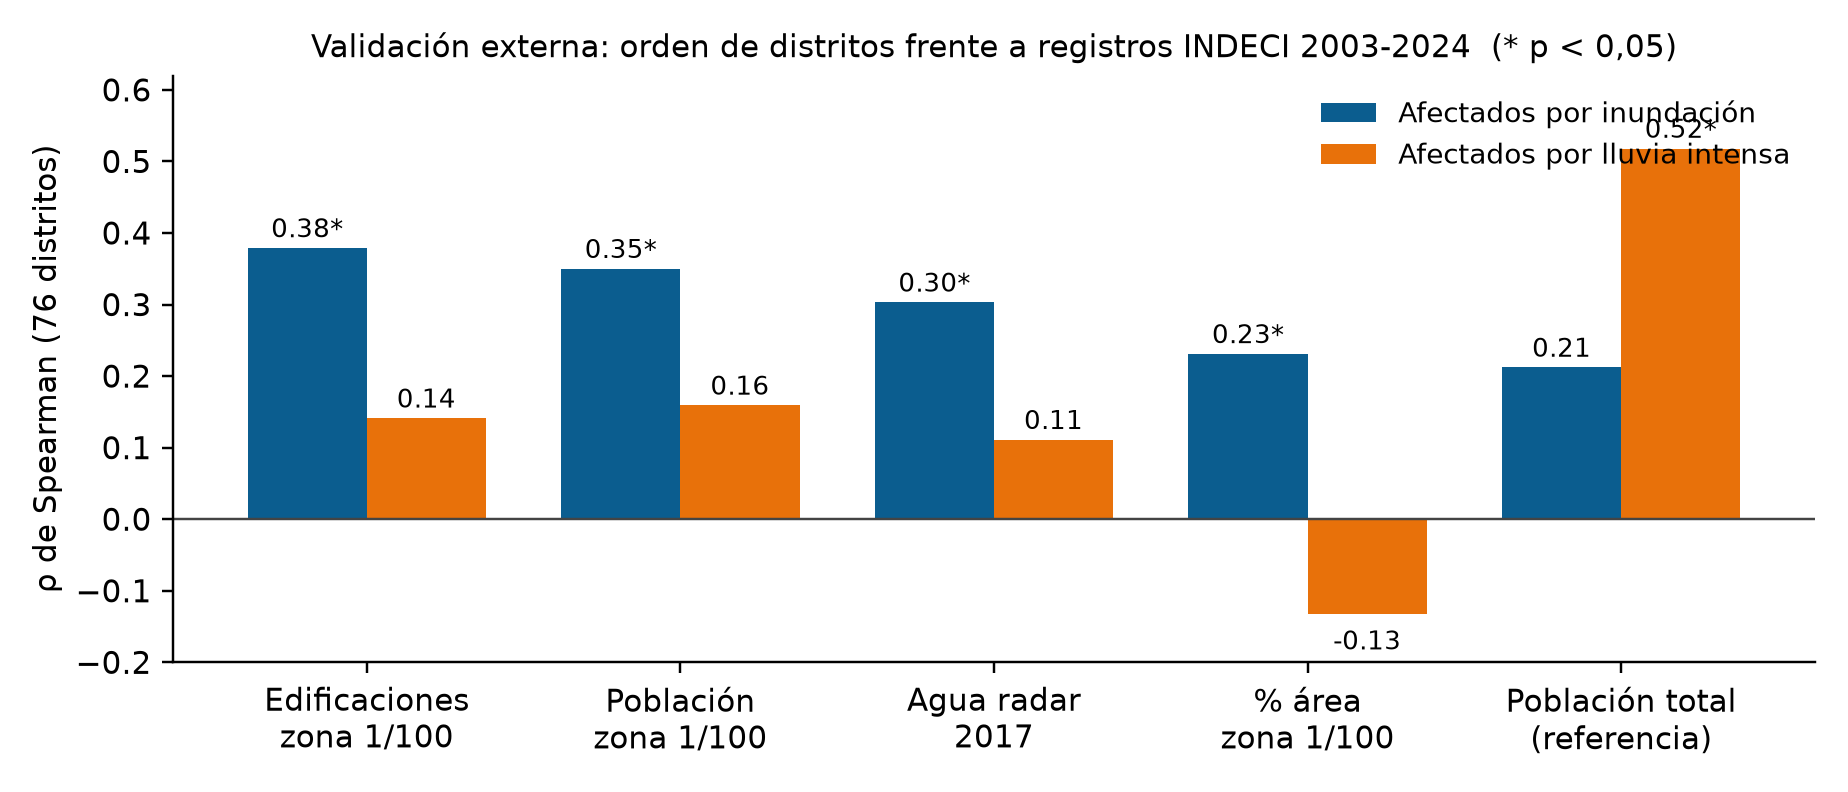
\includegraphics[width=\linewidth]{validacion_indeci.png}
\column{0.36\textwidth}\small
\begin{exampleblock}{Inundación por desborde}
Edificaciones expuestas: $\rho = 0{,}38$ (p < 0,001). Población expuesta: $\rho = 0{,}35$. Ambas superan a la población total ($0{,}21$): la exposición aporta información propia.
\end{exampleblock}
\begin{alertblock}{Lluvia intensa}
La explica la población total ($\rho = 0{,}52$), no la zona inundable fluvial.
\end{alertblock}
\end{columns}
\end{frame}

\begin{frame}{2. Distrito por distrito: ¿acierta el orden?}
\begin{columns}[c]
\column{0.56\textwidth}
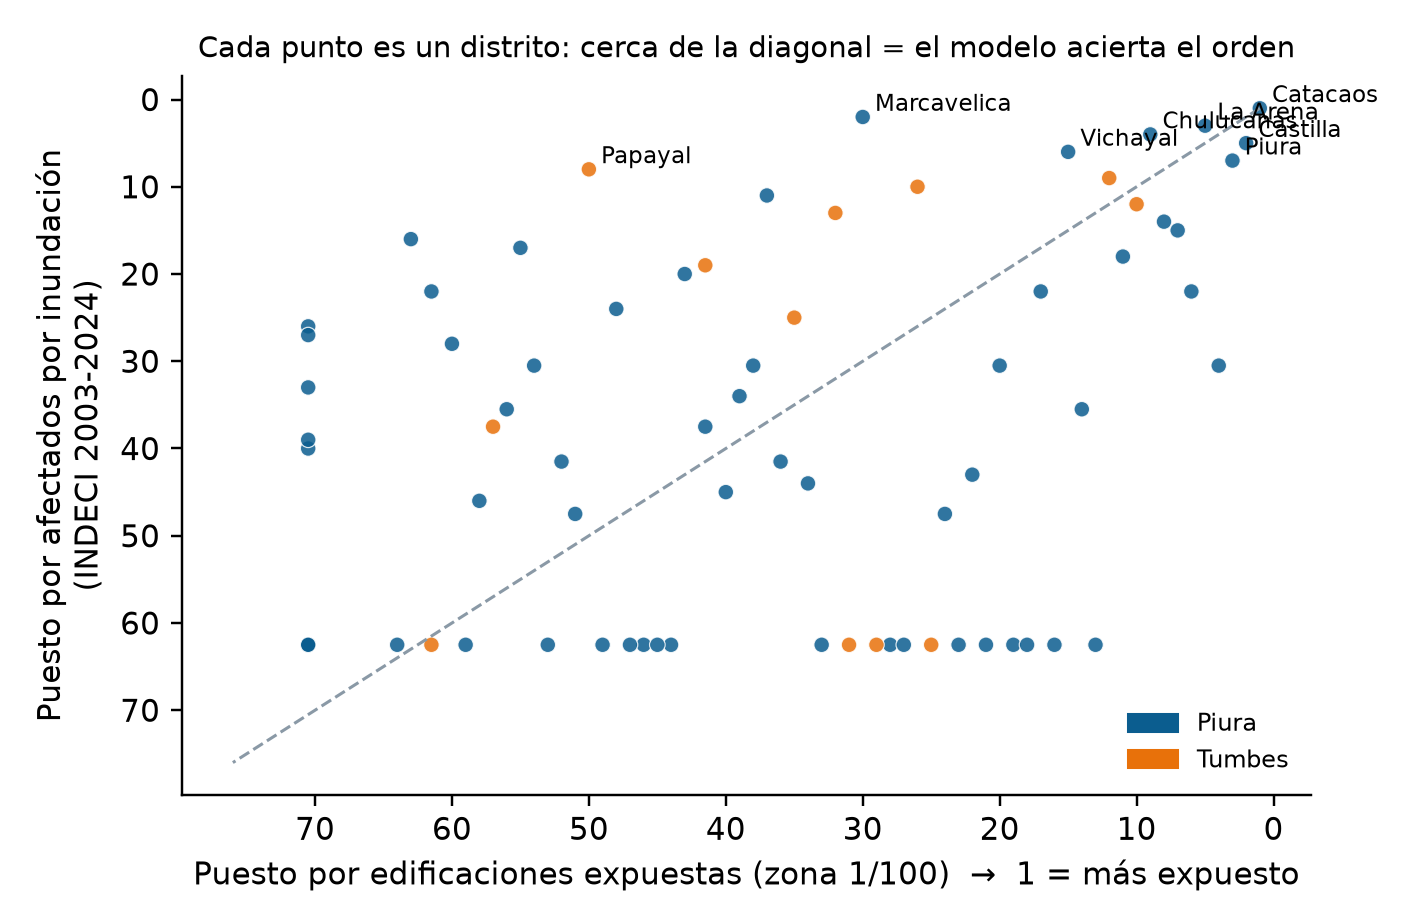
\includegraphics[width=\linewidth]{dispersion_rangos.png}\\
\scriptsize\color{gris} La franja horizontal de abajo son distritos sin afectados por inundación registrados (empatados en el último puesto).
\column{0.42\textwidth}\small
\textbf{Top 15 de INDECI (afectados por inundación y lluvia) frente al top 15 del modelo (población expuesta):}\\[2pt]
\textbf{coinciden 9 de 15}: Castilla, Catacaos, Chulucanas, Colán, La Arena, La Unión, Piura, Tambo Grande y Tumbes.
\vspace{2mm}

\textbf{No los capta el modelo:} Pacaipampa, Yamango, Montero y Las Lomas. Están en la sierra, donde dominan la lluvia intensa y los huaicos.
\end{columns}
\end{frame}

\begin{frame}{3. Lo que todavía no funciona bien}
\begin{columns}[T]
\column{0.32\textwidth}
\begin{alertblock}{Radar en ciudades}\footnotesize
En Catacaos, 2017, solo detectó 1,1 km², aunque fue de los distritos más inundados. El radar con umbral fijo es un \textbf{mínimo}: no ve el agua entre edificios.
\end{alertblock}
\column{0.32\textwidth}
\begin{alertblock}{Alerta semanal (ML)}\footnotesize
No supera con certeza a la climatología: el IC de la diferencia incluye el 0. Captura el 46\,\% de las emergencias de Tumbes y solo el 5\,\% de las de Piura. \textbf{No usarla como alerta.}
\end{alertblock}
\column{0.32\textwidth}
\begin{alertblock}{Índice de riesgo}\footnotesize
$\rho = 0{,}34$ con los afectados por inundación, similar a la exposición sola. Sobrevalora distritos pequeños casi cubiertos por la mancha y sin afectados registrados (Rinconada Llicuar, Bellavista de la Unión).
\end{alertblock}
\end{columns}
\vspace{4mm}
\begin{exampleblock}{Conclusión del piloto}\small
El resultado más sólido es la \textbf{exposición a inundación fluvial por distrito}: está validada en su orden contra una fuente oficial independiente. El radar, el índice compuesto y la alerta semanal necesitan mejoras antes de usarse para decidir.
\end{exampleblock}
\end{frame}

\begin{frame}{4. ¿Es adecuada la base de datos?}
\scriptsize
\renewcommand{\arraystretch}{1.12}
\begin{tabularx}{\textwidth}{L{3.3cm}L{3.2cm}Y}\toprule
\textbf{Componente} & \textbf{¿Adecuado?} & \textbf{Qué falta}\\\midrule
Peligro fluvial (JRC 1/10, 1/100) & \textcolor{ok}{Sí, como base} & Estudios CENEPRED/SIGRID; \textbf{lluvia intensa y huaicos}; defensas ribereñas\\
Población (WorldPop 2026) & \textcolor{ok}{Sí (corregida)} & Censo 2017 y proyecciones oficiales del INEI por distrito o manzana\\
Edificaciones (Open Buildings) & \textcolor{ok}{Sí} & Uso residencial y material de la vivienda (censo)\\
Salud (RENIPRESS) & \textcolor{ok}{Sí} & Verificar coordenadas en campo\\
Colegios (OpenStreetMap) & \textcolor{acento}{No es la ideal} & Padrón ESCALE (MINEDU) con código modular y matrícula\\
Límites (GADM) & \textcolor{acento}{No es la ideal} & Límites oficiales INEI/IGN (faltan 2 distritos; la licencia no permite redistribuir)\\
Vulnerabilidad (pobreza, IDH) & \textcolor{naranja}{Parcial} & Edad, discapacidad, vivienda y saneamiento (Censo 2017)\\
Daños para entrenar (DesInventar) & \textcolor{naranja}{Parcial} & Serie fechada SINPAD 2016--2026\\
Lluvia y caudal (modelados) & \textcolor{naranja}{Parcial} & Estaciones SENAMHI y ANA; avisos oficiales\\\bottomrule
\end{tabularx}
\end{frame}

% ================= PARTE 2 =================
\begin{frame}{5. ¿Cuánto crece el problema?}
\begin{columns}[c]
\column{0.60\textwidth}\small
\renewcommand{\arraystretch}{1.15}
\begin{tabularx}{\linewidth}{YL{0.9cm}L{1.3cm}L{1.1cm}}\toprule
\textbf{Escenario} & \textbf{Dist.} & \textbf{Población} & \textbf{Área}\\\midrule
\textcolor{acento}{\textbf{Piloto}}: Tumbes, Piura & 78 & 2,3 M & 1×\\
\textbf{Norte costero}: + Lambayeque, La Libertad & 199 & 5,8 M & 3,6×\\
\textbf{Norte ampliado}: + Cajamarca, Áncash & 492 & 8,6 M & 4,9×\\
\textbf{Perú}: 25 departamentos & 1\,893 & 34,4 M & 33,5×\\\bottomrule
\end{tabularx}
\vspace{3mm}

\footnotesize\color{gris} Área = caja envolvente que hay que descargar y procesar, comparada con el piloto. Población: estimación 2020 por distrito.
\column{0.36\textwidth}
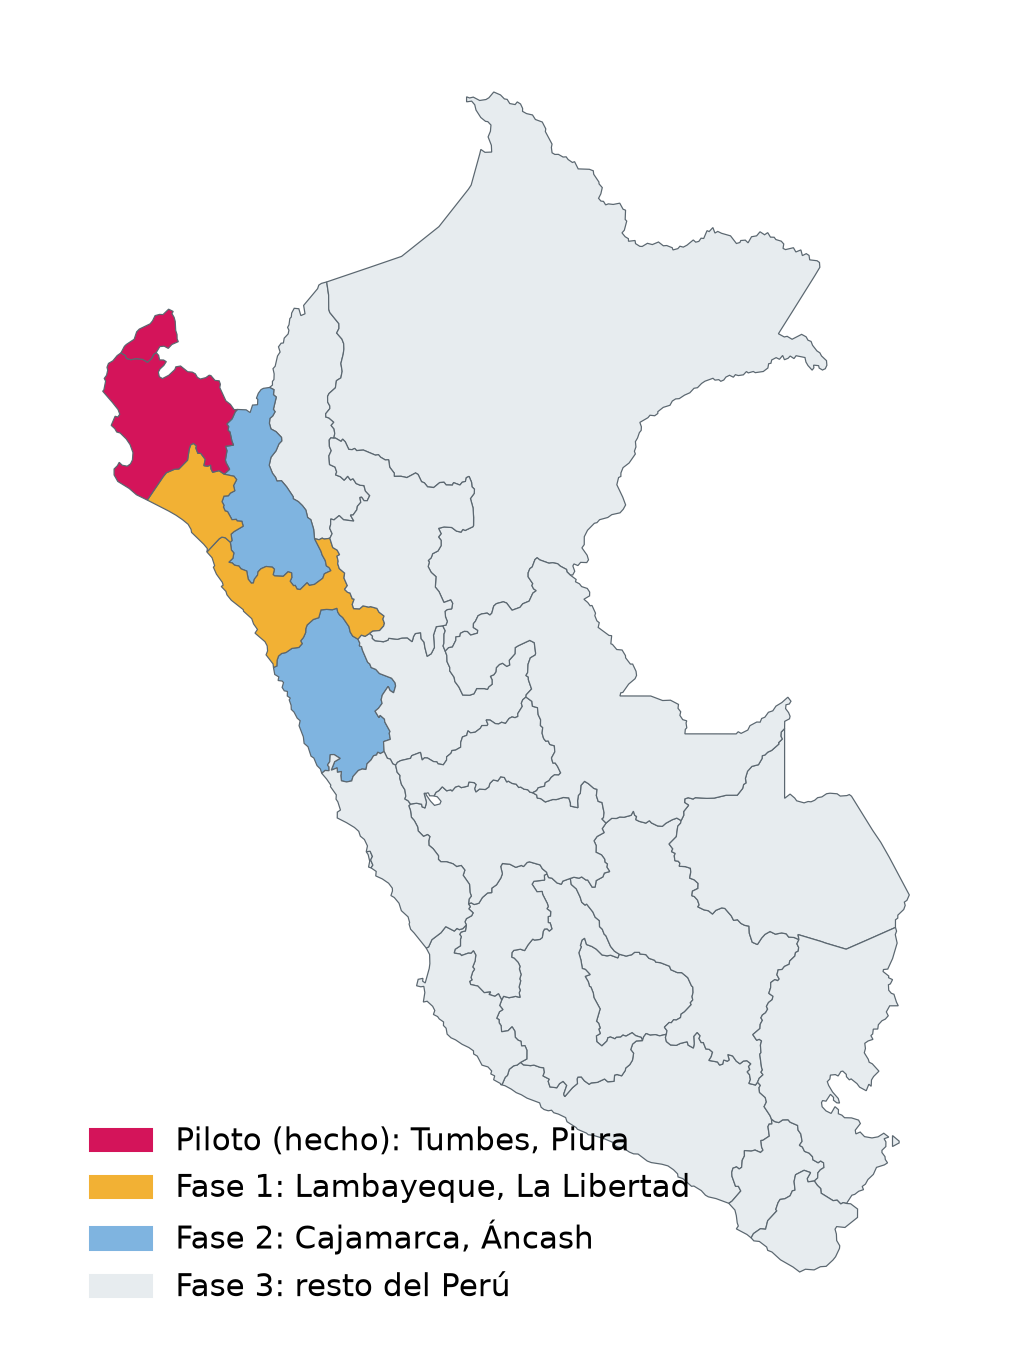
\includegraphics[width=\linewidth]{fases_expansion.png}
\end{columns}
\end{frame}

\begin{frame}{6. Costo de cómputo (con los tiempos medidos en el piloto)}
\begin{columns}[c]
\column{0.58\textwidth}
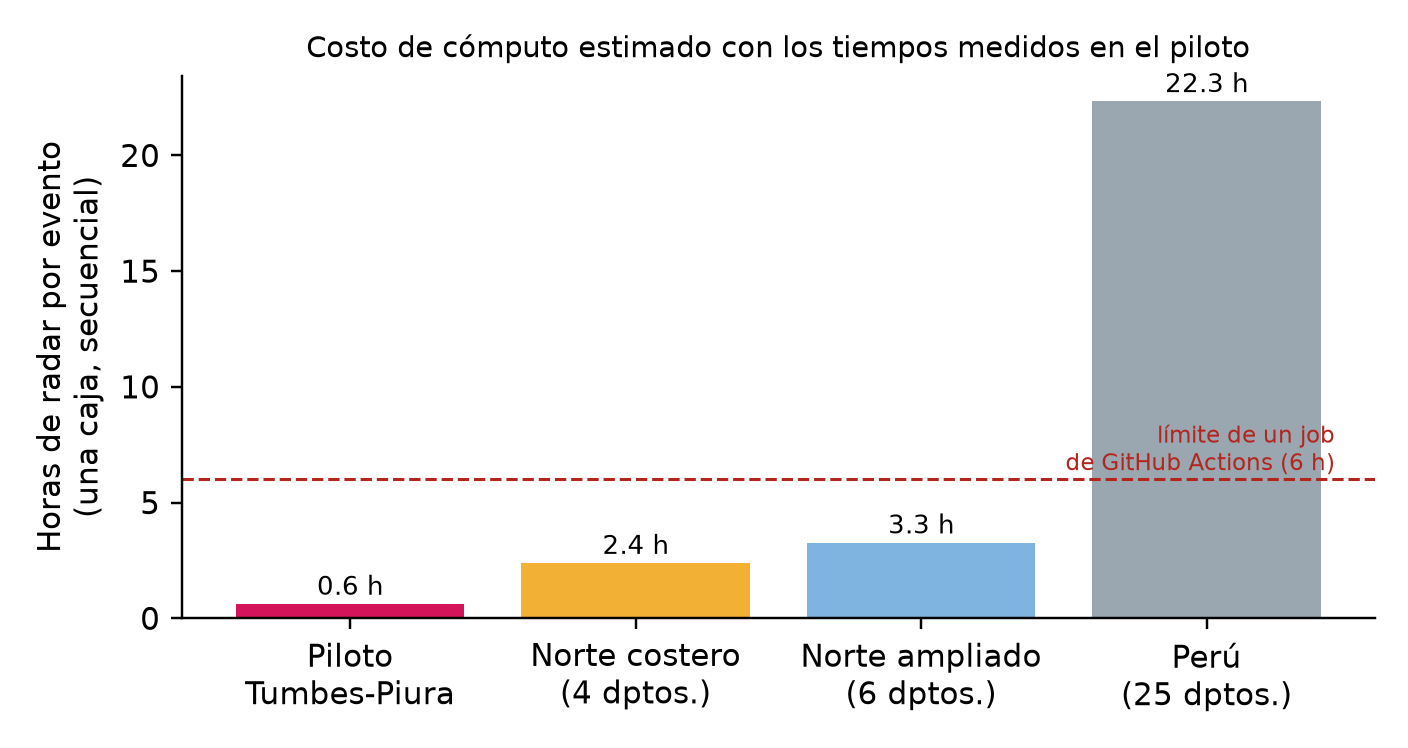
\includegraphics[width=\linewidth]{costo_expansion.png}
\column{0.40\textwidth}\small
\begin{block}{Límites gratuitos de GitHub}\footnotesize
6 h por job · $\sim$16 GB de RAM por runner · sitio de Pages de 1 GB · archivos de hasta 100 MB
\end{block}
\begin{itemize}\footnotesize
\item \textbf{Norte:} cabe en el plan gratuito si se procesa un departamento por job.
\item \textbf{Perú:} 22 h por evento en una sola caja no caben; hay que \textbf{dividir} por departamento o cuenca y correr el radar solo cuando hay un evento.
\item Open Buildings nacional ($\sim$180 MB) supera el límite de 100 MB por archivo: hay que partirlo por departamento.
\end{itemize}
\end{columns}
\end{frame}

\begin{frame}{7. Veredicto de viabilidad}
\begin{columns}[T]
\column{0.32\textwidth}
\begin{exampleblock}{Norte costero}\footnotesize
\textbf{Viable a corto plazo} (1--2 semanas).\\[2pt]
Mismo método y mismas fuentes; la caja y los departamentos pasan a ser parámetros. Es donde El Niño costero golpea más (1983, 1998, 2017, 2023).
\end{exampleblock}
\column{0.32\textwidth}
\begin{block}{Norte ampliado}\footnotesize
\textbf{Viable con ajustes.}\\[2pt]
Cajamarca y Áncash son sobre todo sierra: dominan la lluvia intensa y los huaicos, que el JRC no cubre. Hace falta una capa de peligro adicional (CENEPRED/SIGRID, INGEMMET).
\end{block}
\column{0.32\textwidth}
\begin{alertblock}{Perú completo}\footnotesize
\textbf{Posible, pero con otra arquitectura.}\\[2pt]
Datos y descargas por departamento, mapas en teselas, radar por evento y por cuenca, y otra lógica para la inundación estacional de la Amazonía.
\end{alertblock}
\end{columns}
\vspace{4mm}
\small
\begin{tabularx}{\textwidth}{YL{2.2cm}}\toprule
\textbf{Cambio de código necesario} & \textbf{Esfuerzo}\\\midrule
Caja y departamentos como configuración (no constantes) & 1--2 días\\
Salidas por departamento y selector en el mapa & 2--3 días\\
Workflow con \emph{matrix} por departamento y pruebas parametrizadas & 2 días\\\bottomrule
\end{tabularx}
\end{frame}

\begin{frame}{8. Propuesta para decidir con el docente}
\begin{columns}[T]
\column{0.52\textwidth}
\begin{block}{Ruta recomendada}\small
\begin{enumerate}
\item \textbf{Consolidar el piloto}: límites del INEI, padrón ESCALE, población oficial.
\item \textbf{Agregar el peligro por lluvia intensa y huaicos}, la carencia que mostró la validación.
\item \textbf{Ampliar a la costa norte} (4 departamentos) y repetir la validación con INDECI.
\item Fase posterior: \textbf{cobertura nacional} con la arquitectura por departamento.
\end{enumerate}
\end{block}
\column{0.44\textwidth}
\begin{exampleblock}{Preguntas al docente}\small
\begin{itemize}
\item ¿Priorizamos profundizar la validación en Tumbes y Piura o ampliar ya a la costa norte?
\item ¿Es posible obtener del INEI los límites oficiales y la población por distrito o manzana?
\item ¿Basta la validación de orden con INDECI o se espera una validación con datos de campo?
\end{itemize}
\end{exampleblock}
\end{columns}
\end{frame}

{\setbeamertemplate{footline}{}
\begin{frame}
\begin{tikzpicture}[remember picture,overlay]
\fill[azul] (current page.south west) rectangle (current page.north east);
\node[text=white,align=center] at (current page.center) {{\huge\bfseries Gracias}\\[10pt]
  \large Tablero: \texttt{marciashapiama.github.io/iapn-inei}\\[3pt]
  Mapa 2D: \texttt{marciashapiama.github.io/iapn-inei/mapa2d.html}\\[3pt]
  Reproducir: \texttt{python herramientas/validacion\_indeci.py}\\[1pt]
  \texttt{python herramientas/viabilidad\_expansion.py}};
\end{tikzpicture}
\end{frame}}

\end{document}
